\chapter{Overview}
\label{cha:overview}

This chapter gives informal introduction to the RFSM language and of how to use it to describe 
FSM-based systems.

\medskip
Listing~\ref{lst:rfsm-gensig} is an example of a simple RFSM program\footnote{This program is
  provided in the distribution, under directory \texttt{examples/single/gensig/v2}.}. This program is
used to describe and simulate the model of a calibrated pulse generator. Given an input clock
\verb|H|, with period $T_H$, it generates a pulse of duration $n \times T_H$ whenever input
\texttt{E} is set when event $H$ occurs.

\begin{lstlisting}[language=Rfsm,frame=single,numbers=left,caption=A simple RFSM
  program,label={lst:rfsm-gensig},float]
@\label{gensig-1a}@fsm model gensig <n: int> (
  in h: event,
  in e: bool,
  out s: bool)
{
@\label{gensig-1}@  states: E0 where s=0, E1 where s=1;
  states: E0, E1;
@\label{gensig-3}@  vars: k: int<0:n>;
  trans:
  | E0 -> E1 on h when e=1 with k:=1
@\label{gensig-4}@  | E1 -> E1 on h when k<n with k:=k+1
@\label{gensig-5}@  | E1 -> E0 on h when k=n;
  itrans:
  | -> E0;
@\label{gensig-1b}@}

@\label{gensig-2a}@input H : event = periodic (10,0,80)
input E : bool = value_changes (0:0, 25:1, 35:0)
@\label{gensig-2b}@output S : bool 

@\label{gensig-6}@fsm g = gensig<4>(H,E,S)
\end{lstlisting}

The program can be divided in four parts.

\medskip The first part (lines \ref{gensig-1a}--\ref{gensig-1b}) gives a \textbf{generic model} of
the generator behavior. The model, named \verb|gensig|, has one parameter, \verb|n|, two inputs,
\verb|h| and \verb|e|, of type \verb|event| and \verb|bool| respectively, and one output \verb|s| of
type \verb|bool|. Its behavior is specified as a reactive FSM with two states, \verb|E0| and
\verb|E1|, and one internal variable \verb|k|. The transitions of this FSM are given after the
\verb|trans:| keyword in the form :
\begin{center}
  \framebox{\lstinline[language=Rfsm]{| source_state -> destination_state on ev when guard with actions}}
\end{center}
where
\begin{itemize}
\item \emph{ev} is the event trigerring the transition,
\item \emph{guard} is a set of (boolean) conditions,
\item \emph{actions} is a set of actions performed when the transition is enabled.
\end{itemize}

The semantics is that the transition is enabled
whenever the FSM is in the source state, the event \emph{ev} occurs and all the conditions in the
guard are true. The associated actions
are then performed and the FSM moves to the destination state. For example, the first transition is
enabled whenever an event occurs on input \verb|h| and, at this instant, the value of input \verb|e|
is 1. The FSM then goes from state \verb|E0| to state \verb|E1| and sets its internal variable 
\verb|k|.
   
The \emph{initial transition} of the FSM is given 
after the \verb|itrans:| keyword in the form :
\begin{center}
  \framebox{\lstinline[language=Rfsm]{| -> initial_state with actions}}
\end{center}
Here the FSM is initially in state \verb|E0|.

The value of the \texttt{s} output is attached to states, using
the \lstinline[language=Rfsm]{where} keyword~: this value is 0 when the
system is in state \texttt{E0} and 1 when the system is in state \texttt{E1}.

\textbf{Note}. In the transitions, the \lstinline[language=Rfsm]{when guard} and
\lstinline[language=Rfsm]{with actions} are optional and may be omitted.

A graphical representation of the \verb|gensig| model is given in
Fig.~\ref{fig:rfsm-gensig-model} (this representation was actually automatically generated from the
program in Listing~\ref{lst:rfsm-gensig}, as explained in Chap.~\ref{cha:rfsmc}). 

\begin{figure}[!h]
   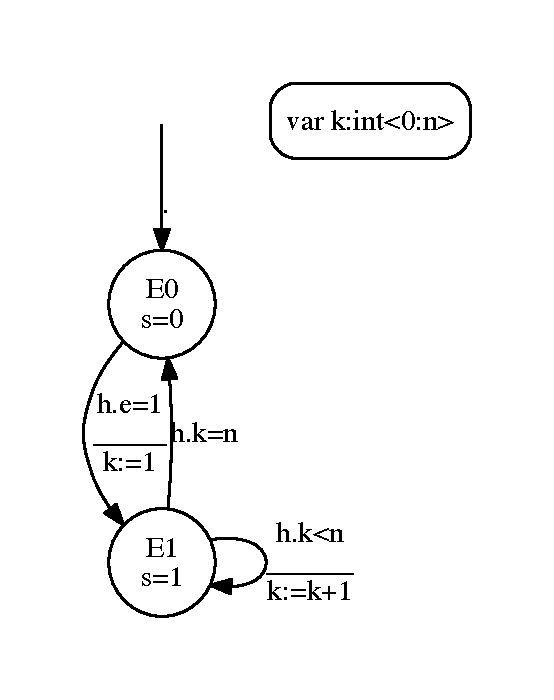
\includegraphics[height=8cm]{figs/gensig-model}
   \centering
  \caption{A graphical representation of FSM model defined in Listing~\ref{lst:rfsm-gensig}}
  \label{fig:rfsm-gensig-model}
\end{figure}

Note that, at this level, the value of the parameter \verb|n|, used in the type of the internal
variable \verb|k| (line~\ref{gensig-3}) and in the transition conditions (lines \ref{gensig-4} and
\ref{gensig-5}) is left unspecified, making the \verb|gensig| model a \emph{generic} one.

\medskip The second part of the program (lines \ref{gensig-2a}--\ref{gensig-2b}) lists \textbf{global inputs and
  outputs}\footnote{In case of multi-FSM programs, this part will also contains the declaration of
  \emph{shared} events and variables. See Sec.~\ref{sec:globals}.}.  For global outputs the
declaration simply gives a name and a type.  For global inputs, the declaration also specifies the
\textbf{stimuli} which are attached to the corresponding input for simulating the system. The
program of Listing~\ref{lst:rfsm-gensig} uses two kinds of stimuli\footnote{See
  Sec.~\ref{sec:globals} for a complete description of stimuli.}. The stimuli attached to input
\verb|H| are declared as \emph{periodic}, with a period of 10 time units, a start time of 0 and a
end time of 80. This means than an event will be produced on this input at time 0, 10, 20, 30, 40,
50, 60, 70 and 80. The stimuli attached to input \verb|E| say that this input will respectively take
value 0, 1 and 0 at time 0, 25 and 35 (thus producing a ``pulse'' of duration 10 time units starting
at time 25).

\medskip
The third and last part of the program (line~\ref{gensig-6}) consists in building the global model of the system by
\emph{instanciating} the FSM model(s).
Instanciating a model creates a ``copy'' of this model for which
\begin{itemize}
\item the generic parameters (\verb|n| here) are now bound to actual values (4 here),
\item the inputs and outputs are connected to the global inputs or outputs. 
\end{itemize}

\medskip
A graphical representation of the system described in Listing~\ref{lst:rfsm-gensig} is given in
Fig.~\ref{fig:rfsm-gensig-top}\footnote{Again, this representation was actually automatically generated from the
program in Listing~\ref{lst:rfsm-gensig}, as explained in Chap.~\ref{cha:rfsmc}}. 

\begin{figure}[!h]
   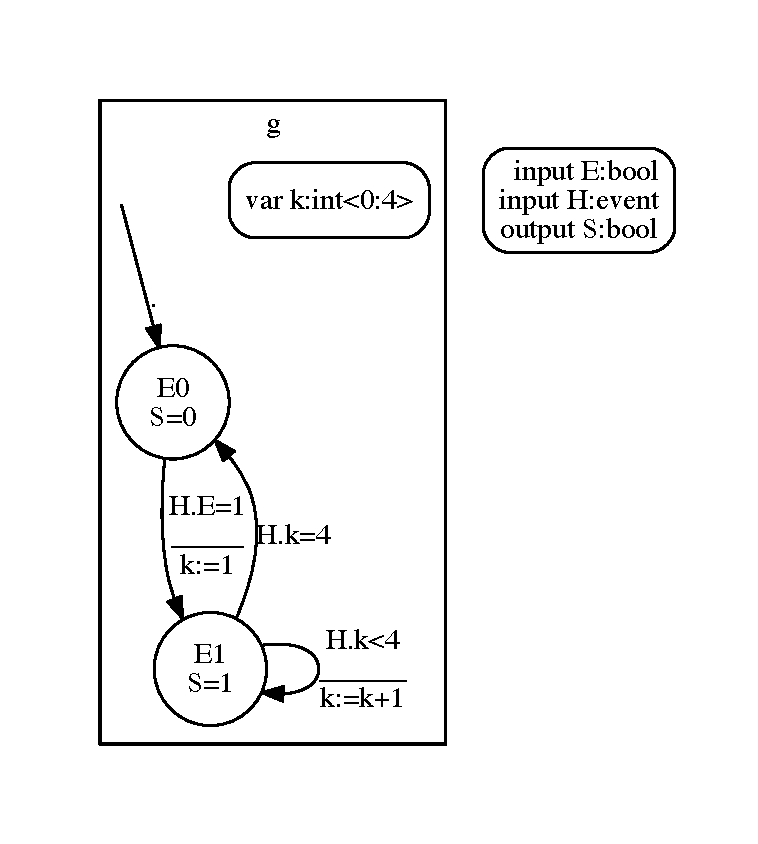
\includegraphics[height=8cm]{figs/gensig-top}
   \centering
  \caption{A graphical representation of system described in Listing~\ref{lst:rfsm-gensig}}
  \label{fig:rfsm-gensig-top}
\end{figure}

\section*{Simulating}
\label{sec:simulating-1}

Simulating the program means computing the reaction of the system to the input stimuli. Simulation
can be performed the RFSM command-line compiler or the IDE (see Chap.~\ref{cha:rfsmc} and \ref{cha:gui} resp.).
It produces a set of
\emph{traces} in VCD (Value Change Dump) format which can visualized using \emph{waveform viewers}
such as \texttt{gtkwave}. The simulation results for the program in Listing~\ref{lst:rfsm-gensig}
are illustrated in Fig.~\ref{fig:rfsm-gensig-chrono}.

\begin{figure}[!h]
   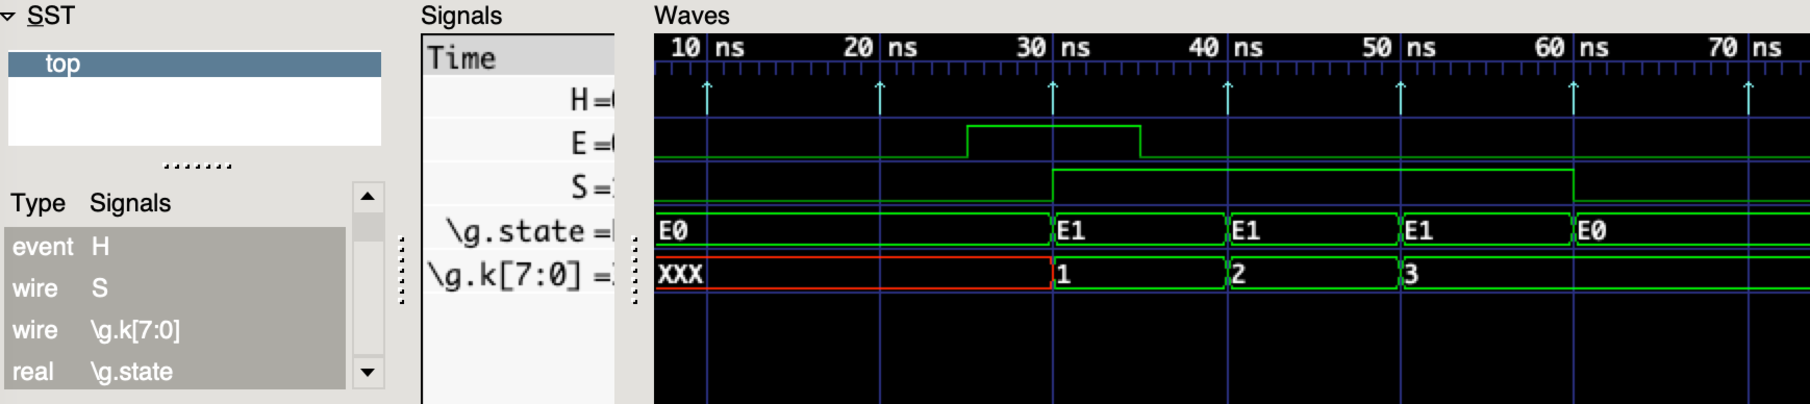
\includegraphics[width=\textwidth]{figs/gensig-chrono}
   \centering
  \caption{Simulation results for the program in Listing~\ref{lst:rfsm-gensig}, viewed using
    \texttt{gtkwave}}
  \label{fig:rfsm-gensig-chrono}
\end{figure}

\section*{Code generation}
\label{sec:code-generation-1}

RFSM can also generate code implementing the described systems simulation and/or
integration to existing applications.

\medskip
Currently, three backends are provided :
\begin{itemize}
\item a backend generating a C-based implementation of each FSM instance,
\item a backend generating a \emph{testbench} implementation in SystemC (FSM instances + stimuli
  generators),
\item a backend generating a \emph{testbench} implementation in VHDL (FSM instances + stimuli
  generators).
\end{itemize}

\medskip
The target language for the C backend is a C-like language augmented with
\begin{itemize}
\item a \verb|task| keyword for naming generated behaviors,
\item \verb|in|, \verb|out| and \verb|iinout| keywords for identifying inputs and outputs,
\item a builtin \verb|event| type,
\item primitives for handling events : \verb|wait_ev()|, \verb|wait_evs()| and
  \verb|notify_ev()|. 
\end{itemize}
The idea is that the generated code can be turned into an application for a multi-tasking operating
system by providing actual implementations of the corresponding constructs and primitives.

\medskip
For the SystemC and VHDL backends, the generated code can actually be compiled and executed for
simulation purpose and. The FSM implementations generated by the VHDL backend can also be
synthetized to be implemented hardware using hardware-specific tools\footnote{We use the
  \textsc{quartus} toolchain from Intel/Altera.}. 

\medskip
Appendices C1, C2 and C3 respectively give the C and SystemC code generated from the example in
Listing~\ref{lst:rfsm-gensig}. 

\section*{Variant formulation}
\label{sec:variant-formulation}

In the automata described in Fig.~\ref{fig:rfsm-gensig-model} and Listing~\ref{lst:rfsm-gensig}, the
\texttt{s} output is defined by attaching its value to states.
This is typical of a so-called \emph{Moore}-style description.
Iy is also possible to specify these values by indicating how they are \emph{modified} when some
transitions are taken. A equivalent description of that given in Listing~\ref{lst:rfsm-gensig} is
obtained, for example, by specifying that
\texttt{s} is set to 0 on the initial transition and on the transition from \texttt{E1} to
\texttt{E0}, and set to 1 on the transition from \texttt{E0} to \texttt{E1}. 
This style of description, often called \emph{Mealy}-style, is illustrated in
Fig.~\ref{fig:rfsm-gensig-mealy} and
Listing~\ref{lst:rfsm-gensig-mealy}. Note the absence of the \texttt{where} clause in the
declarations of states at line~\ref{gensigm-1} and, conversely, the presence of the action
\lstinline[language=Rfsm]{s:=0} and \lstinline[language=Rfsm]{s:=1} at lines~\ref{gensigm-3} and
\ref{gensigm-2b}, and \ref{gensigm-2a} respectively.

\begin{figure}[!h]
   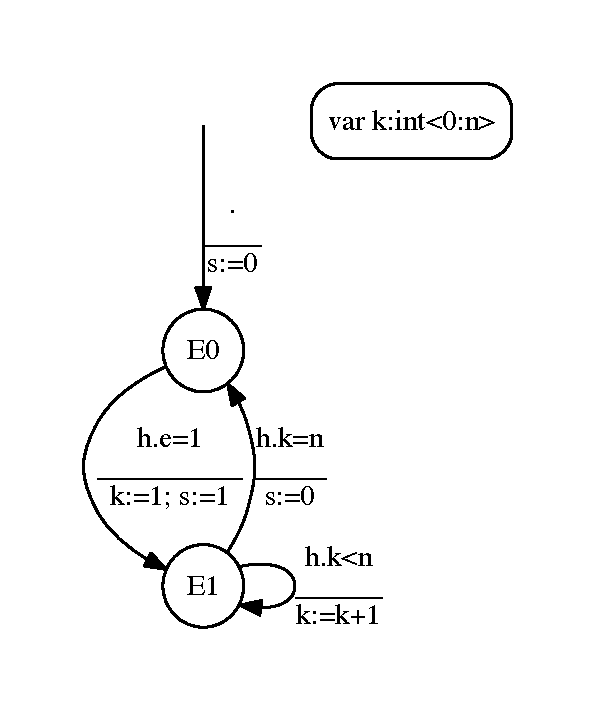
\includegraphics[height=6cm]{figs/gensig-model-mealy}
   \centering
  \caption{A Mealy-style reformulation of the model defined in Fig.~\ref{fig:rfsm-gensig-model}}
  \label{fig:rfsm-gensig-mealy}
\end{figure}

\begin{lstlisting}[language=Rfsm,frame=single,numbers=left,caption=Transcription in RFSM of the
  model given in Fig.~\ref{fig:rfsm-gensig-mealy},label={lst:rfsm-gensig-mealy},float]
fsm model gensig <n: int> (
  in h: event,
  in e: bool,
  out s: bool)
{
@\label{gensigm-1}@  states: E0, E1;
  vars: k: int<0:n>;
  trans:
@\label{gensigm-2a}@  | E0 -> E1 on h when e=1 with k:=1, s:=1
  | E1 -> E1 on h when k<n with k:=k+1
@\label{gensigm-2b}@  | E1 -> E0 on h when k=n, s:=0
  itrans:
@\label{gensigm-3}@  | -> E0 with s:=0
}
\end{lstlisting}

\medskip \textbf{Note}. An option of the \texttt{rfsmc} compiler (\verb|-normalize|) allows to
automatically transform a Moore-style description into a Mealy-style one.
% This option is
% automatically inserted when simulating a system\footnote{\emph{I.e.} simulation is always performed
%   on Mealy-style FSMs.}. 


%%% Local Variables: 
%%% mode: latex
%%% TeX-master: "rfsm"
%%% End: 
